\newpage
\section{Dynamic Programming}
\subsection{Divide and Conquer}
\begin{figure}[H]
    \centering
    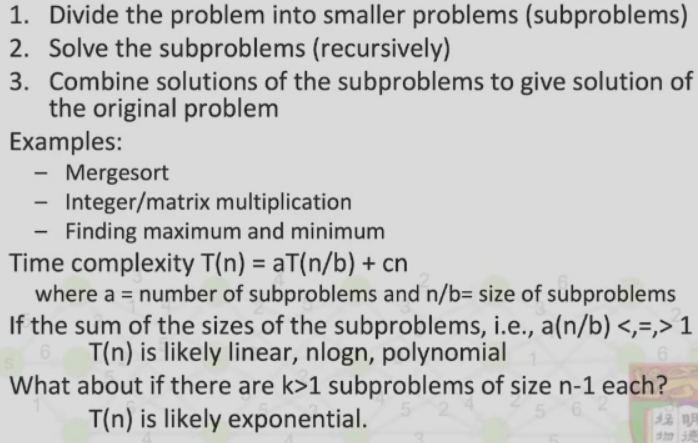
\includegraphics[width=0.309\textwidth]{pic/DAA8/Divide and Conquer}
    \caption{Divide and Conquer}
\end{figure}

\subsection{Multistage Graph}
\begin{figure}[H]
    \centering
    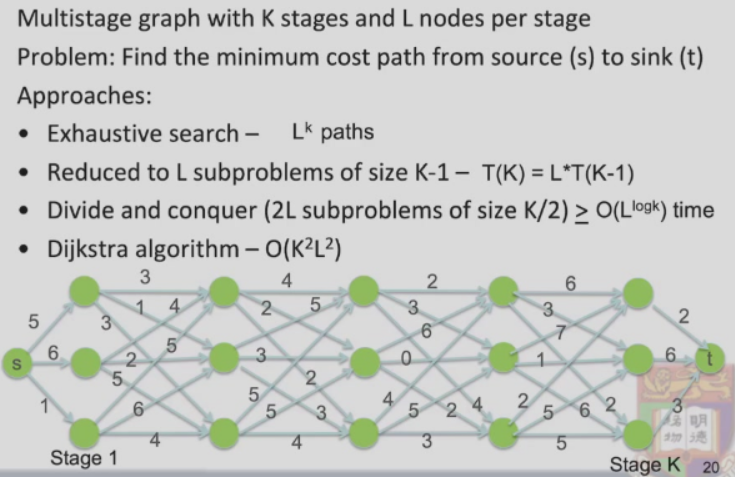
\includegraphics[width=0.309\textwidth]{pic/DAA8/Multistage Graph}
    \caption{Shortest Path Problem}
\end{figure}

\begin{figure}[H]
    \centering
    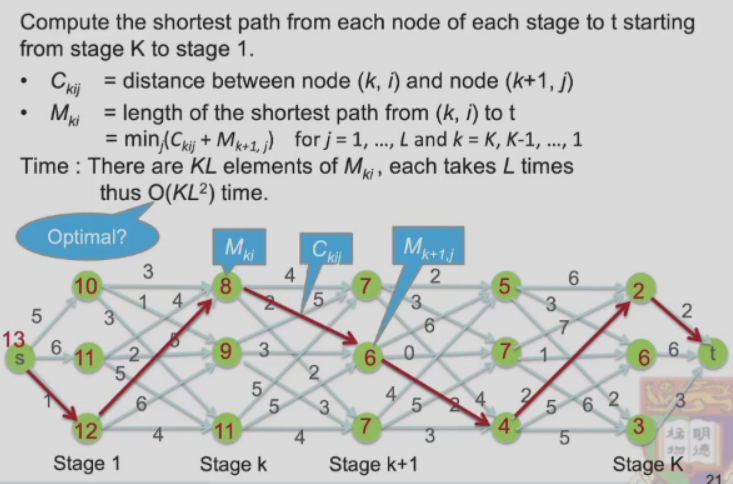
\includegraphics[width=0.309\textwidth]{pic/DAA8/Multistage Graph - DP}
    \caption{Multistage Graph - DP}
\end{figure}
Optimal

\subsubsection{DP Implementation}
\begin{figure}[H]
    \centering
    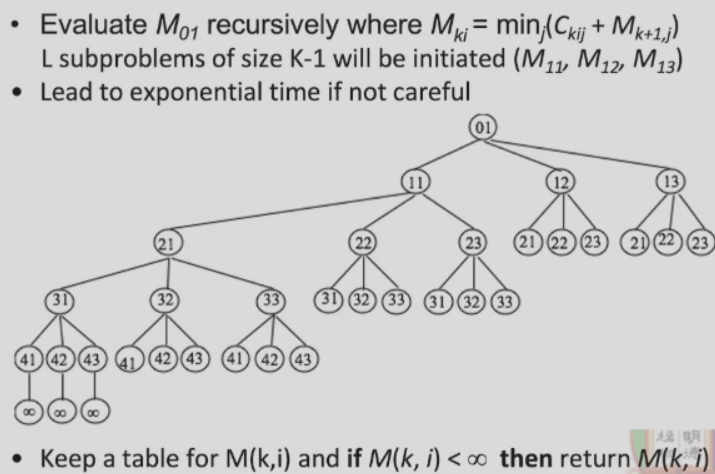
\includegraphics[width=0.309\textwidth]{pic/DAA8/DP Implementation}
    \caption{DP Implementation}
\end{figure}

\subsection{Principle of Optimality}
\begin{figure}[H]
    \centering
    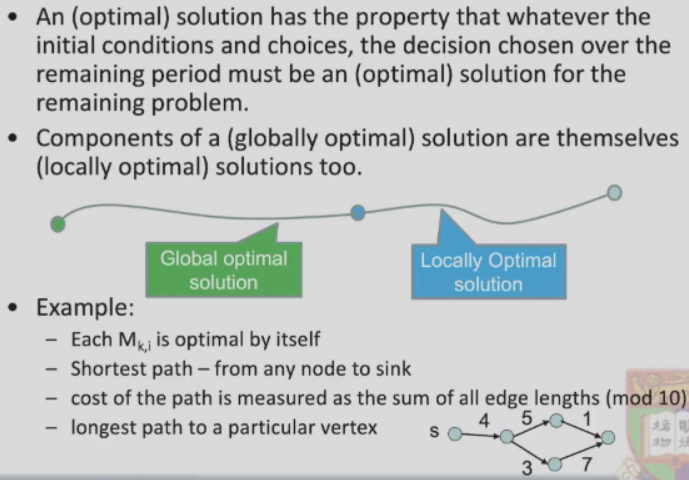
\includegraphics[width=0.309\textwidth]{pic/DAA8/Principle of Optimality}
    \caption{Principle of Optimality}
\end{figure}

\subsubsection{integer Decomposition}
\begin{figure}[H]
    \centering
    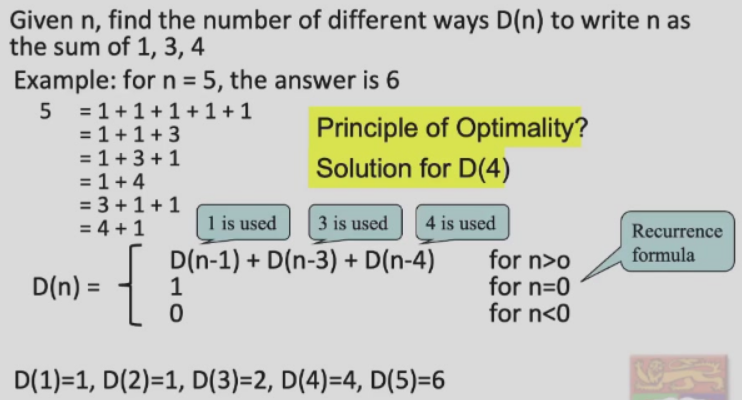
\includegraphics[width=0.309\textwidth]{pic/DAA8/integer Decomposition}
    \caption{integer Decomposition}
\end{figure}

\subsubsection{Number of Tilings}
\begin{figure}[H]
    \centering
    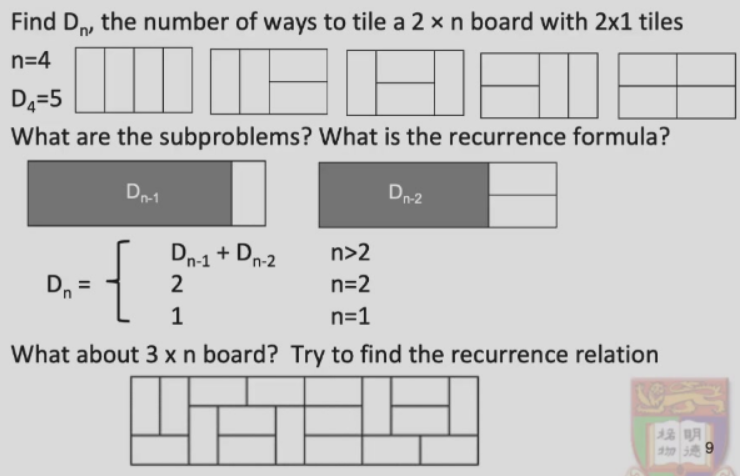
\includegraphics[width=0.309\textwidth]{pic/DAA8/Number of Tilings}
    \caption{Number of Tilings}
\end{figure}

\subsection{How to Solve Problems by DP}

\begin{figure}[H]
    \centering
    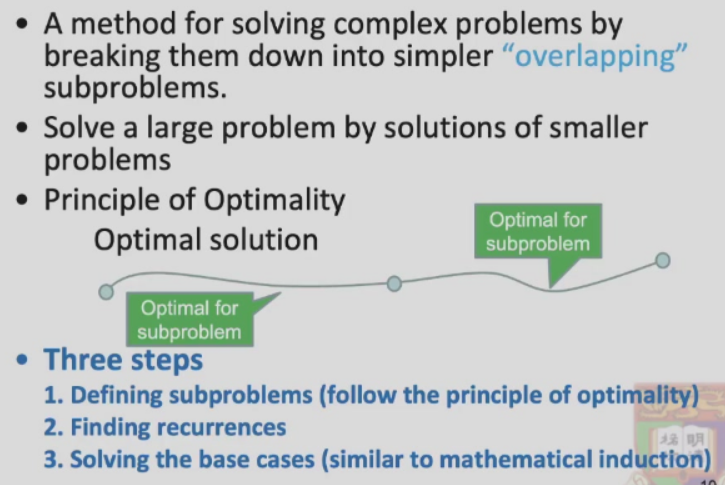
\includegraphics[width=0.309\textwidth]{pic/DAA8/How to Solve Problems by DP}
    \caption{How to Solve Problems by DP}
\end{figure}

\subsubsection{Longest Common Subsequence}
% \begin{figure}[H]
%     \centering
%     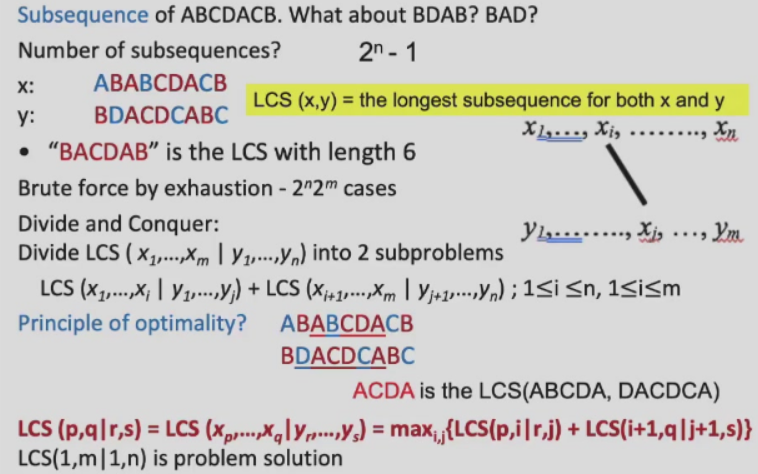
\includegraphics[width=0.309\textwidth]{pic/DAA8/Longest Common Subsequence}
%     \caption{Longest Common Subsequence}
% \end{figure}

\begin{figure}[H]
    \centering
    \begin{subfigure}{0.309\textwidth}
        \centering
        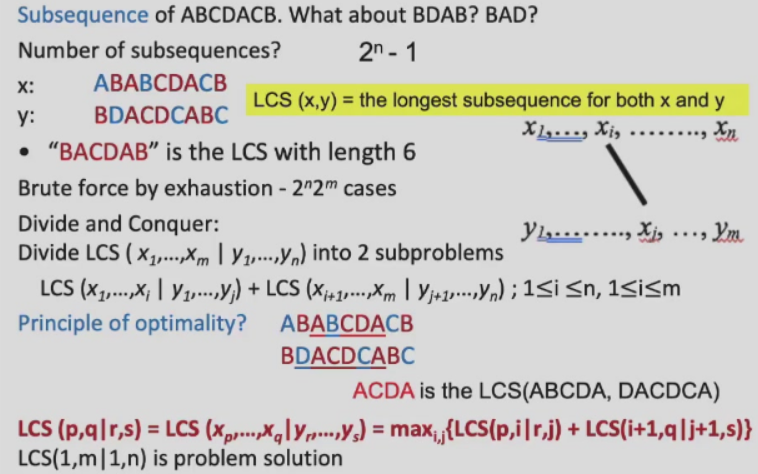
\includegraphics[width=\textwidth]{pic/DAA8/Longest Common Subsequence}
        % \caption{}
    \end{subfigure}
    \begin{subfigure}{0.309\textwidth}
        \centering
        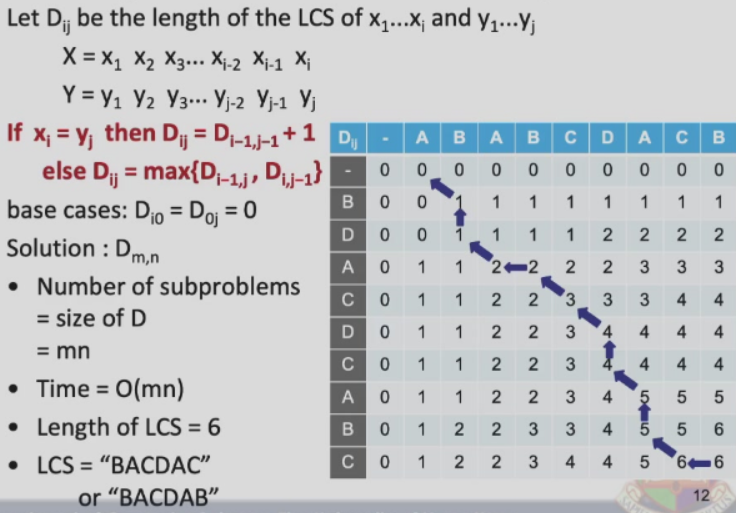
\includegraphics[width=\textwidth]{pic/DAA8/Longest Common Subsequence1}
        % \caption{}
    \end{subfigure}
    \caption{Longest Common Subsequence}
\end{figure}

\subsubsection{Palindrome Problem}

\begin{figure}[H]
    \centering
    \begin{subfigure}{0.309\textwidth}
        \centering
        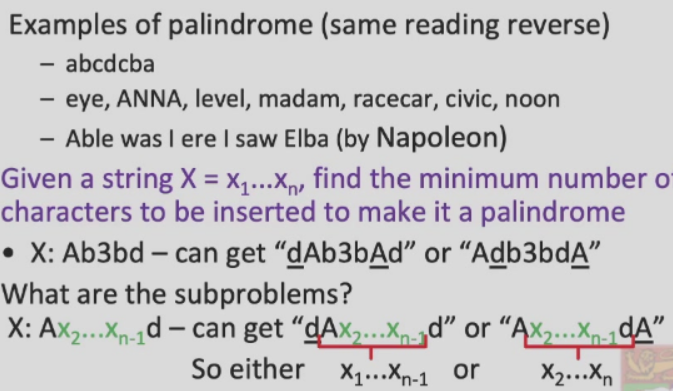
\includegraphics[width=\textwidth]{pic/DAA8/Palindrome Problem}
        % \caption{}
    \end{subfigure}
    \begin{subfigure}{0.309\textwidth}
        \centering
        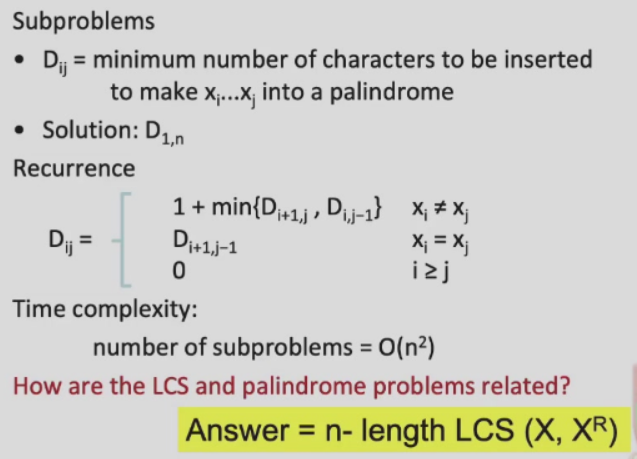
\includegraphics[width=\textwidth]{pic/DAA8/Palindrome Problem1}
        % \caption{}
    \end{subfigure}
    \caption{Palindrome Problem}
\end{figure}


\subsubsection{Longest Increasing Subsequence}

\begin{figure}[H]
    \centering
    \begin{subfigure}{0.309\textwidth}
        \centering
        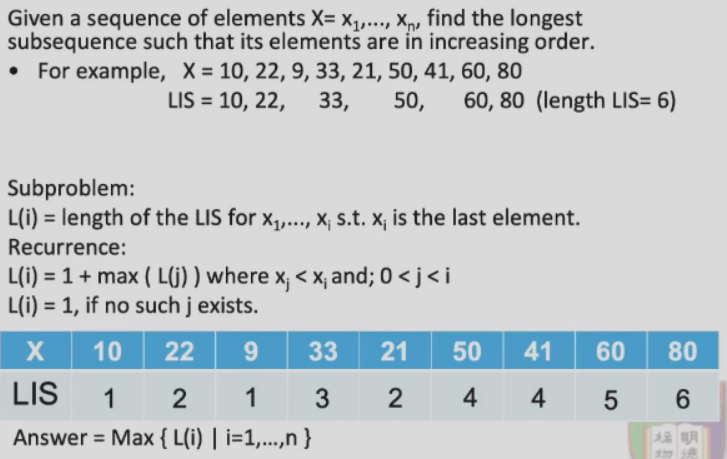
\includegraphics[width=\textwidth]{pic/DAA8/Longest Increasing Subsequence}
        % \caption{}
    \end{subfigure}
    \begin{subfigure}{0.309\textwidth}
        \centering
        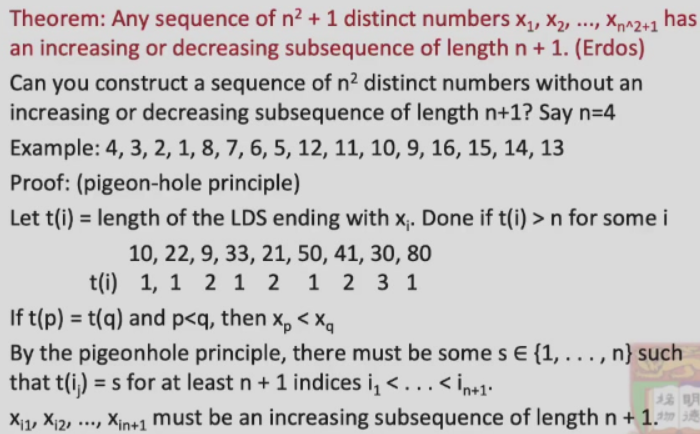
\includegraphics[width=\textwidth]{pic/DAA8/Longest Increasing Subsequence1}
        % \caption{}
    \end{subfigure}
    \caption{Longest Increasing Subsequence}
\end{figure}

\subsubsection{Tree Coloring}
\begin{figure}[H]
    \centering
    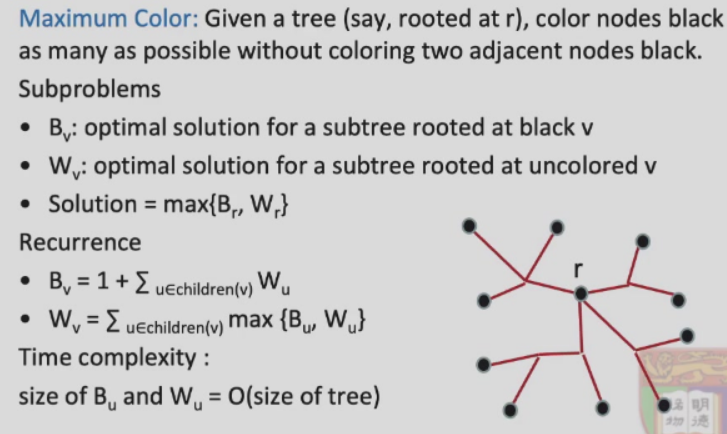
\includegraphics[width=0.309\textwidth]{pic/DAA8/Tree Coloring}
    \caption{Tree Coloring}
\end{figure}

\subsubsection{Traveling Salesman Problem}
\begin{figure}[H]
    \centering
    \begin{subfigure}{0.309\textwidth}
        \centering
        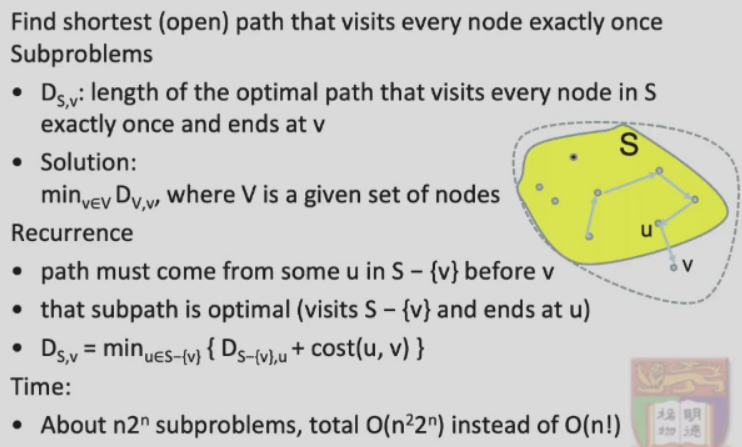
\includegraphics[width=\textwidth]{pic/DAA8/Traveling Salesman Problem}
        % \caption{}
    \end{subfigure}
    \begin{subfigure}{0.309\textwidth}
        \centering
        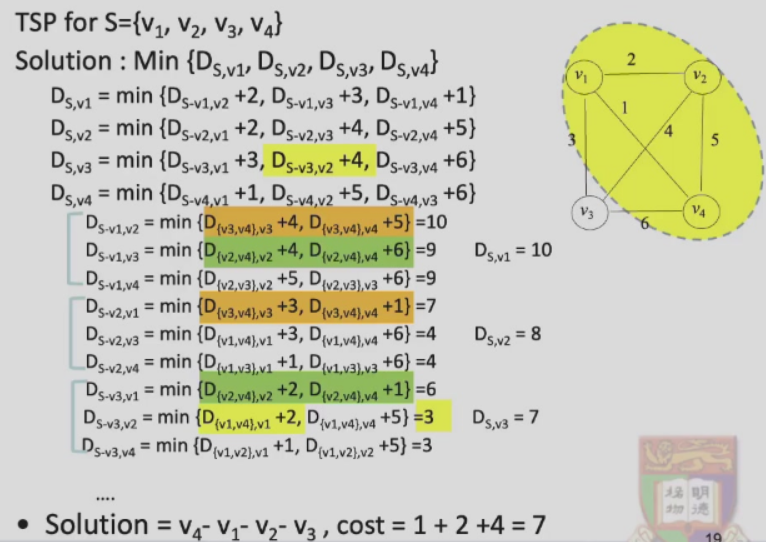
\includegraphics[width=\textwidth]{pic/DAA8/Traveling Salesman Problem1}
        % \caption{}
    \end{subfigure}
    \caption{Traveling Salesman Problem}
\end{figure}

